%!TEX root = ../talk.tex

\section{TensorFlow}\label{sec:TF}

%%%

\frameinlbffalse

{
\usebackgroundtemplate{
\tikz[overlay,remember picture] \node[opacity=0.8, xshift=-3.5cm, at=(current page.east)] {

\includegraphics[width=0.35\paperwidth]{figures/TF_logo.png}
};}

\begin{frame}[plain]
\frametitle{\S\ref{sec:TF}. \insertsection}
\listofframes
\end{frame}
\addtocounter{framenumber}{-1} % this page does not count

}

\frameinlbftrue

%%%
\subsection{Programming interface}
%%%

\begin{frame}
  \MyLogo
  \frametitle{Basic Concepts}
  \begin{itemize}
	  	\item Graph: In TensorFlow, ML algorithms are represented as computational graph. A computational graph (data flow graph) is a form of directed graph where vertices (nodes) describe operations, while edges represent data flowing between these operations.
	  	
	  	\item Operation: An operation may represent a variable or constant, a control flow directive, a mathematical function, a file I/O, or a network communication port.
	  	
	  	\item Tensor: A tensor is a multi-dimensional collection of homogeneous values with a fixed static type.
	  	
	  	\item Variable: Variables can be described as persistent, mutable handles to in-memory buffers storing tensors.
	  	
	  	\item Session: In TensorFlow the execution of operations and evaluation of tensors may only be preformed in a special environment called session.
	  	
\end{itemize}

\end{frame}

%%%
\subsection{Computational graph}
%%%

\begin{frame}[fragile]
  \MyLogo
  \frametitle{Computational Graph}  
%  
\begin{columns}
\column{.65\textwidth}
\tiny{
\begin{lstlisting}[language=python]
import tensorflow as tf

graph = tf.Graph()

with graph.as_default():
	# Define two constants
	a = tf.constant(1.0)
	b = tf.constant(2.0)

	# Define an operation node: c = a * b
	c = tf.multiply(a, b)
	# Add scalar summary to operation node
	tf.summary.scalar('c', c)
	
	# Merge all the summaries and write to ./board
	merged = tf.summary.merge_all()
	writer = tf.summary.FileWriter('./board', graph)

with tf.Session(graph=graph):
	# Write data to ./board
	writer.add_summary(merged.eval())
	
\end{lstlisting}
}
\column{.2\textwidth}
%
\begin{figure}[htbp] 
   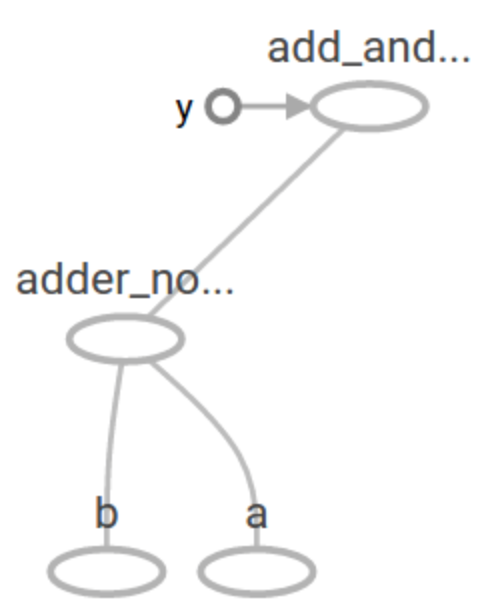
\includegraphics[height=2.5in]{figures/compgraph.png} 
\end{figure}
%
\end{columns}
\end{frame}

%%%
\subsection{Simple examples}
%%%

\begin{frame}[fragile]
  \MyLogo
  \frametitle{Example: SoftMax in TF}  
 
\begin{lstlisting}[language=python]
import tensorflow as tf

# Import training and test data
import tensorflow.examples.tutorials.mnist.input_data as input_data
mnist = input_data.read_data_sets("MNIST_data/", one_hot=True)

# Create a new TensorFlow graph
graph = tf.Graph()
with graph.as_default():
	# Nodes or entire subgraphs can be grouped into one visual block for tensorboard
	with tf.name_scope('input_features'):
		# Placeholder for input variables (None = variable dimension)
		x = tf.placeholder(tf.float32, shape=[None, 784], name='input_x')
							
	with tf.name_scope('input_labels'):
		# Placeholder for labels
		y_ = tf.placeholder(tf.float32, shape=[None, 10], name='labels')
							
	with tf.name_scope('parameters'):
		W = tf.Variable(tf.zeros([784, 10]), name='weights')
		# Track tensor distributions over time for tensorboard
		tf.summary.histogram('WEIGHTS', W)
		b = tf.Variable(tf.zeros([10]), name='biases')
		tf.summary.histogram('BIASES', b)
			
	with tf.name_scope('use_softmax'):
		# Apply softmax regression model to the input data and get prediction y
		y = tf.nn.softmax(tf.matmul(x, W) + b)
\end{lstlisting}

\end{frame}

\begin{frame}[fragile]
  \MyLogo
  \frametitle{Example: SoftMax in TF (Cont)}  

\ContinueLineNumber
\begin{lstlisting}[language=python]
	with tf.name_scope('train'):
		# Compute the cross entropy of real label y_ and prediction labe y
		cross_entropy = -tf.reduce_sum(y_*tf.log(y))
		# Create a gradient-descent optimizer with learning rate = 0.01
		train_step = tf.train.GradientDescentOptimizer(0.01).minimize(cross_entropy)

	with tf.name_scope('test'):
		correct_prediction = tf.equal(tf.argmax(y,1), tf.argmax(y_,1))
		accuracy = tf.reduce_mean(tf.cast(correct_prediction, "float"))
		# Track tensor values over time for tensorboard
		tf.summary.scalar('Accuracy', accuracy)
	
	merged = tf.summary.merge_all()   # Merge all the summaries
	writer = tf.summary.FileWriter('./board', graph)  # Write summary file to ./board
	
with tf.Session(graph=graph) as sess:
	# Initialize all variables
	tf.global_variables_initializer().run()
	
	for step in range(1000):
		if (step%10) == 0:
			# Feed test data to compute accuarcy
			feed = {x: mnist.test.images, y_: mnist.test.labels}
			_, acc = sess.run([merged, accuracy], feed_dict=feed)
			print('Accuracy at %s step: %s' %(step, acc))
		else:
			# Feed training data to train the model
			batch_x, batch_y = mnist.train.next_batch(100)
			sess.run(train_step, feed_dict={x: batch_x, y_: batch_y})
			writer.add_summary(merged.eval(feed_dict={x:batch_x, y_:batch}),
							   global_step=step)
\end{lstlisting}

\end{frame}

%%%
\subsection{Visualization}
%%%

\begin{frame}[fragile]
  \MyLogo
  \frametitle{Visualization: TensorBoard}  

\vskip -25pt
\begin{columns}
\column{.48\textwidth}  
\scriptsize{
\structure{Declarative style}
\begin{itemize}
\item  Same style as Teano
\item  Easy to understand
\item  Possible for graph optimization
\item  More difficult for debugging
\end{itemize}

\medskip

\structure{Computation graphs are powerful but complicated}
\begin{itemize}
\item  Thousands of nodes or more 
\item  Network is deep
\item  Visualization is helpful for debugging 
\end{itemize}
}
%
\column{.48\textwidth}
\begin{figure}[htbp] 
   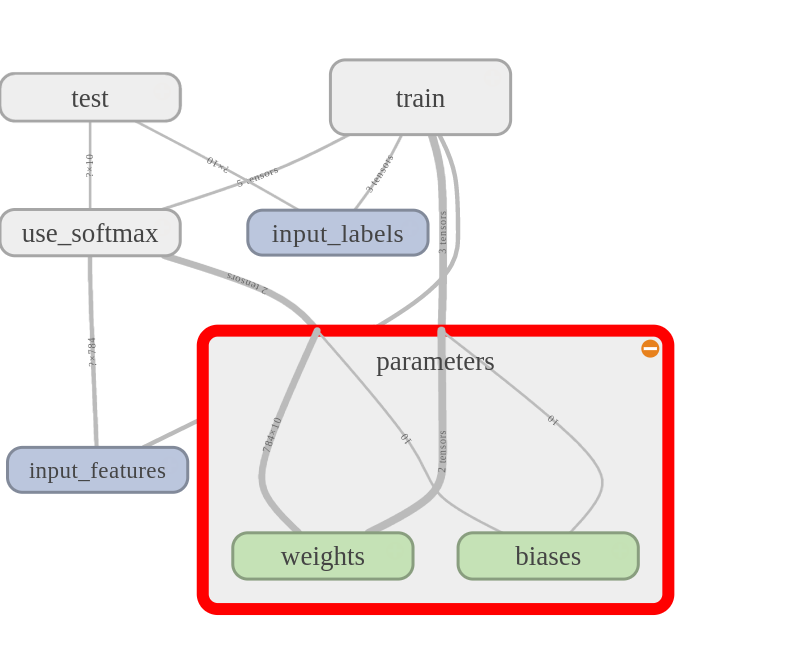
\includegraphics[height=2.2in]{figures/graphvisualization.png} 
\end{figure}
\end{columns}

To run TensorBoard, use the following command: 
\begin{lstlisting}[language=sh,numbers=none] 
$ tensorboard --logdir=path/to/log-directory
\end{lstlisting}
Then navigate your web browser to localhost:6006 to view the TensorBoard.

\end{frame}

%

\begin{frame}
	\MyLogo
	\frametitle{TensorBoard: Scalars}  

\centering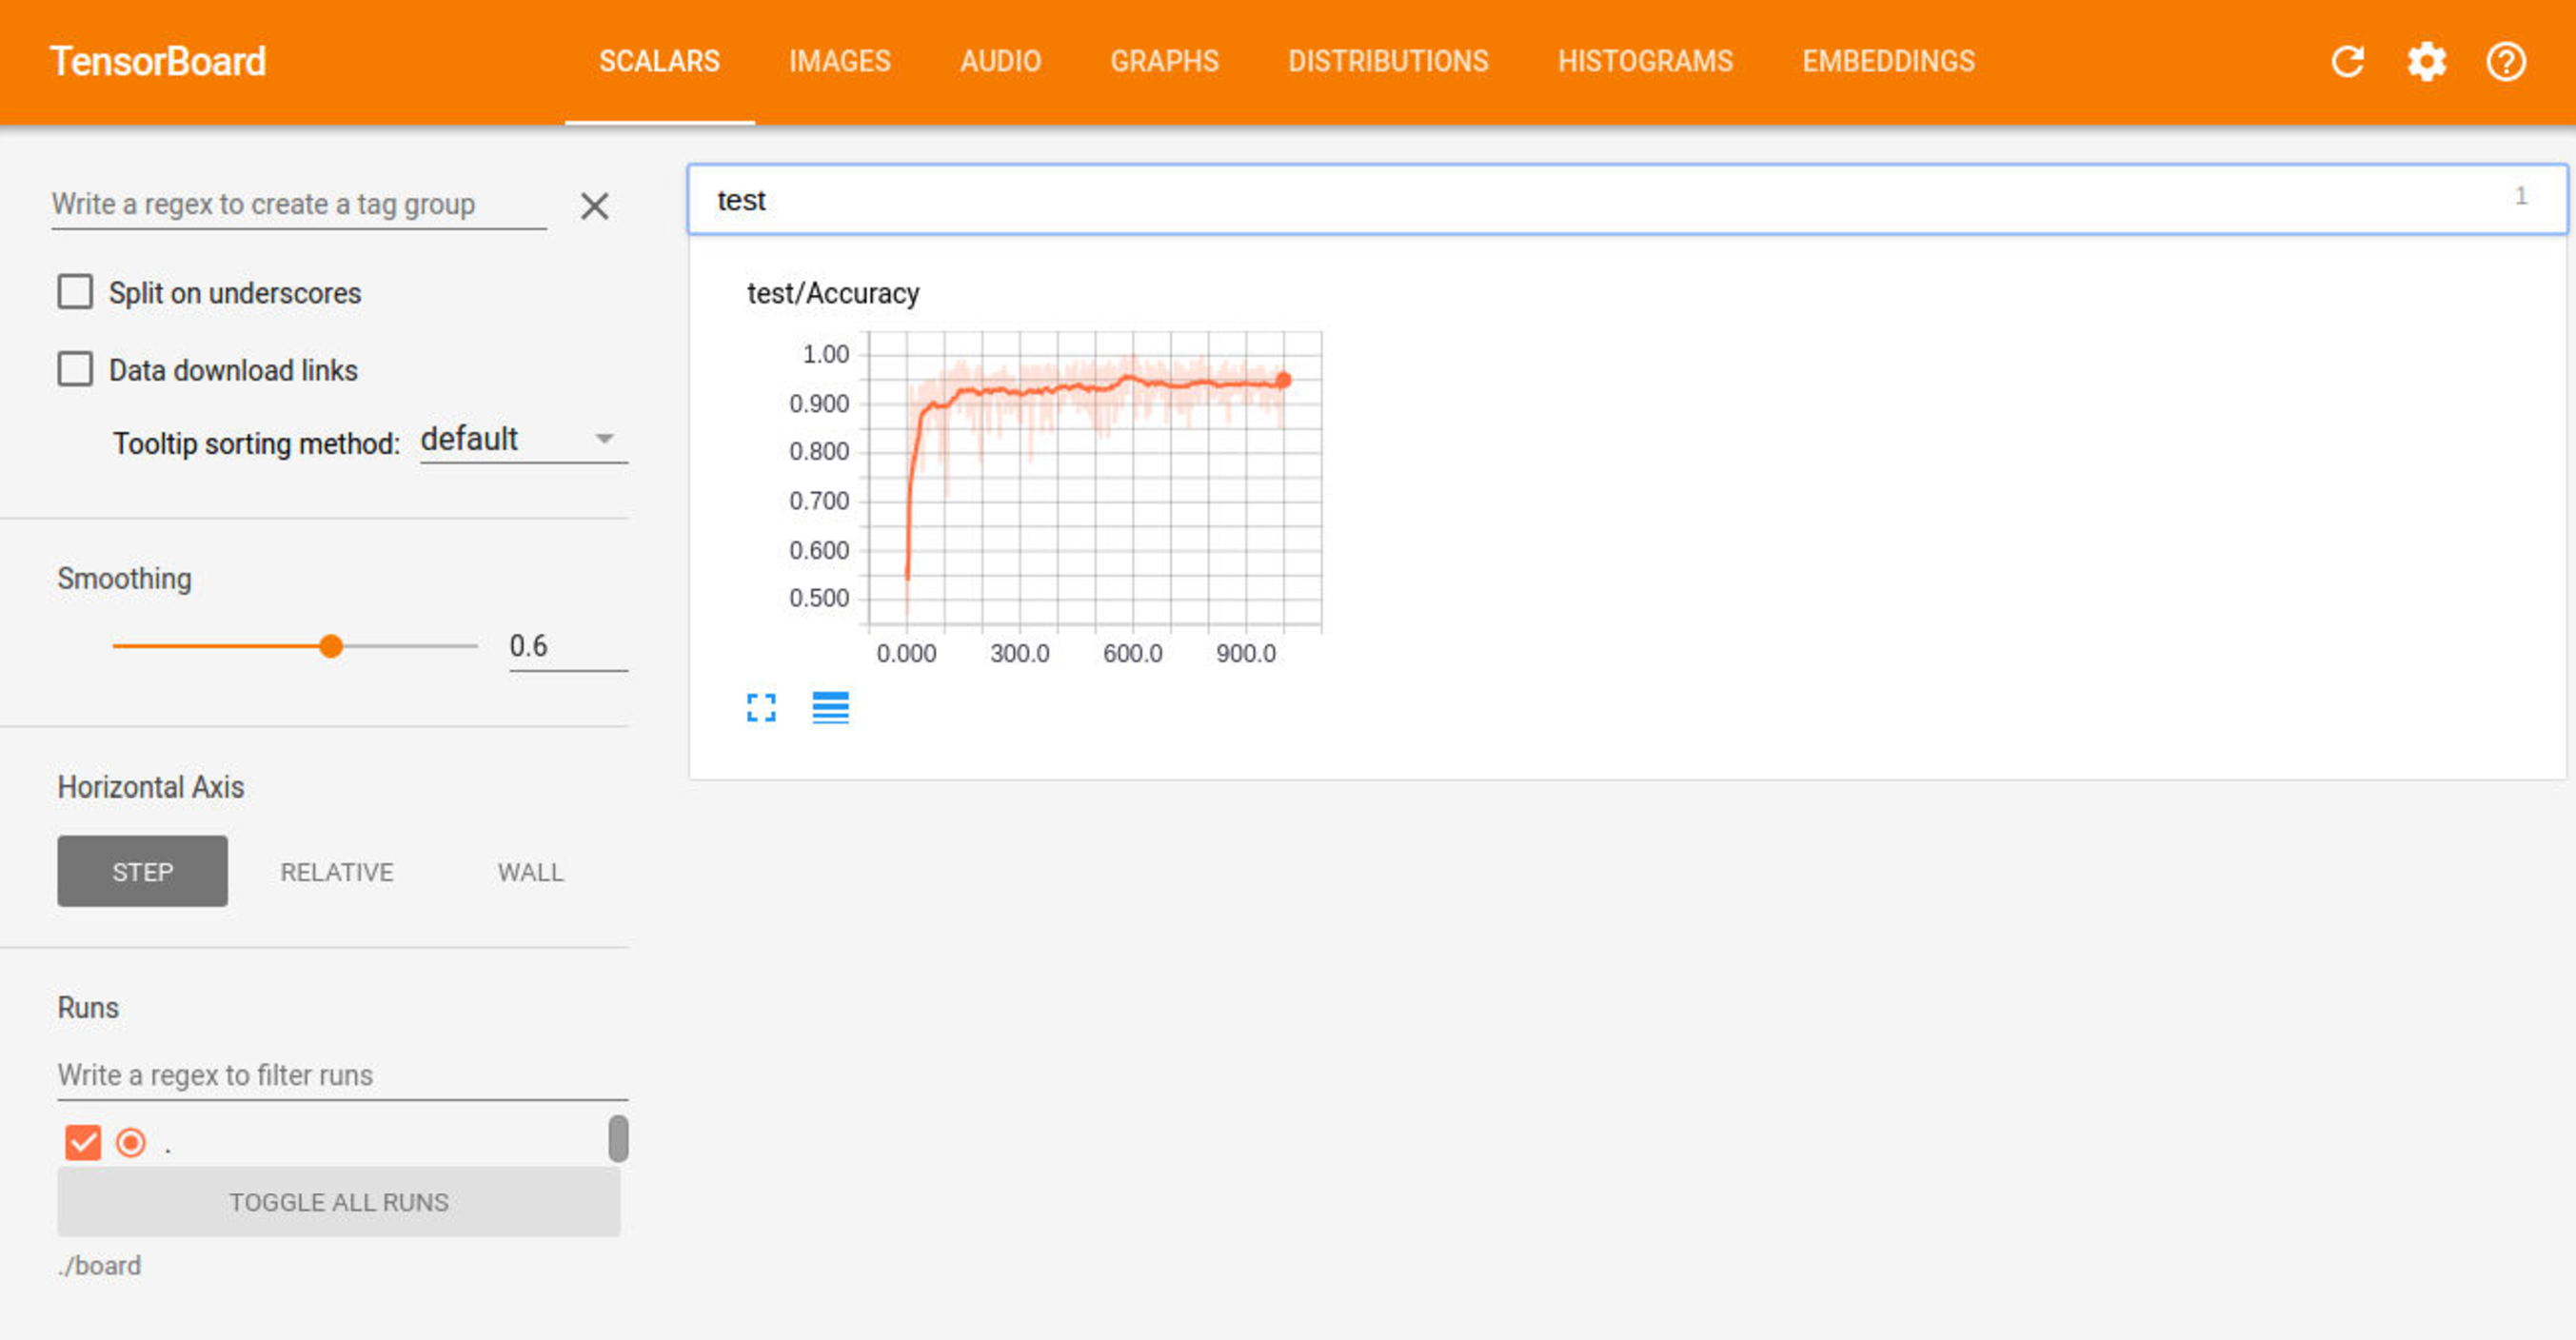
\includegraphics[width=0.95\paperwidth]{figures/scalar.pdf} 
	
\end{frame}

%

\begin{frame}
	\MyLogo
	\frametitle{TensorBoard: Graphs}  
	
\centering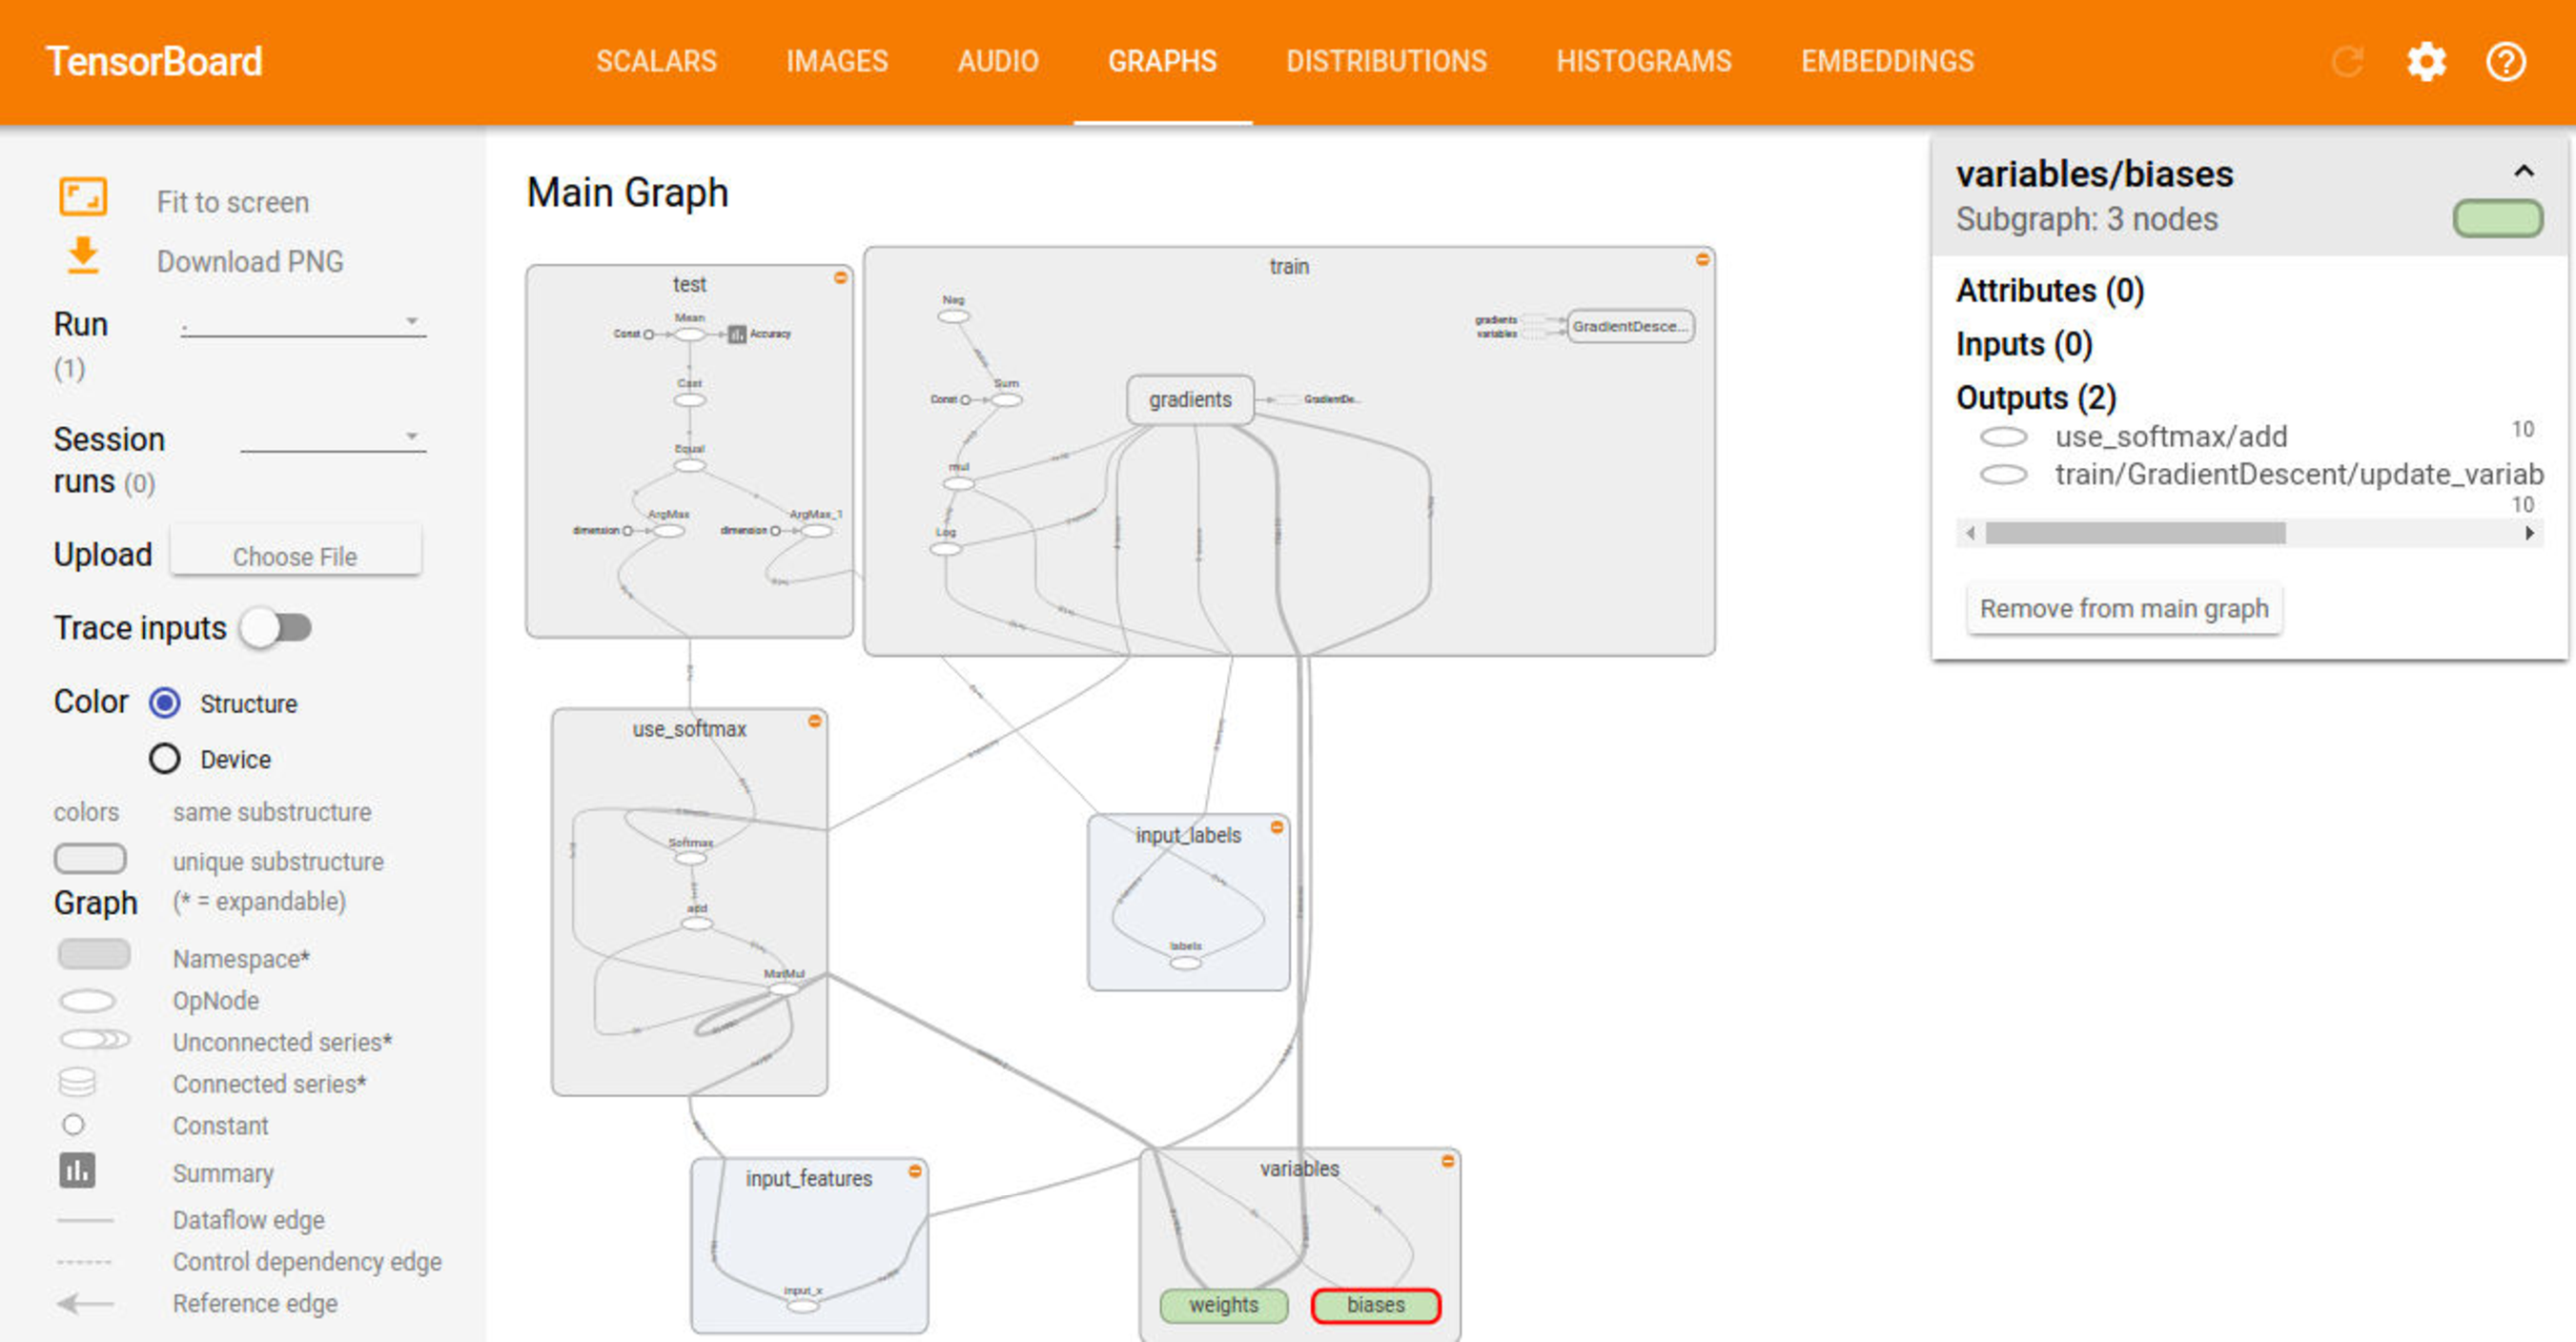
\includegraphics[width=0.95\paperwidth]{figures/main_graph.pdf} 
	
\end{frame}

%

\begin{frame}
	\MyLogo
	\frametitle{TensorBoard: Distributions}  
	
\centering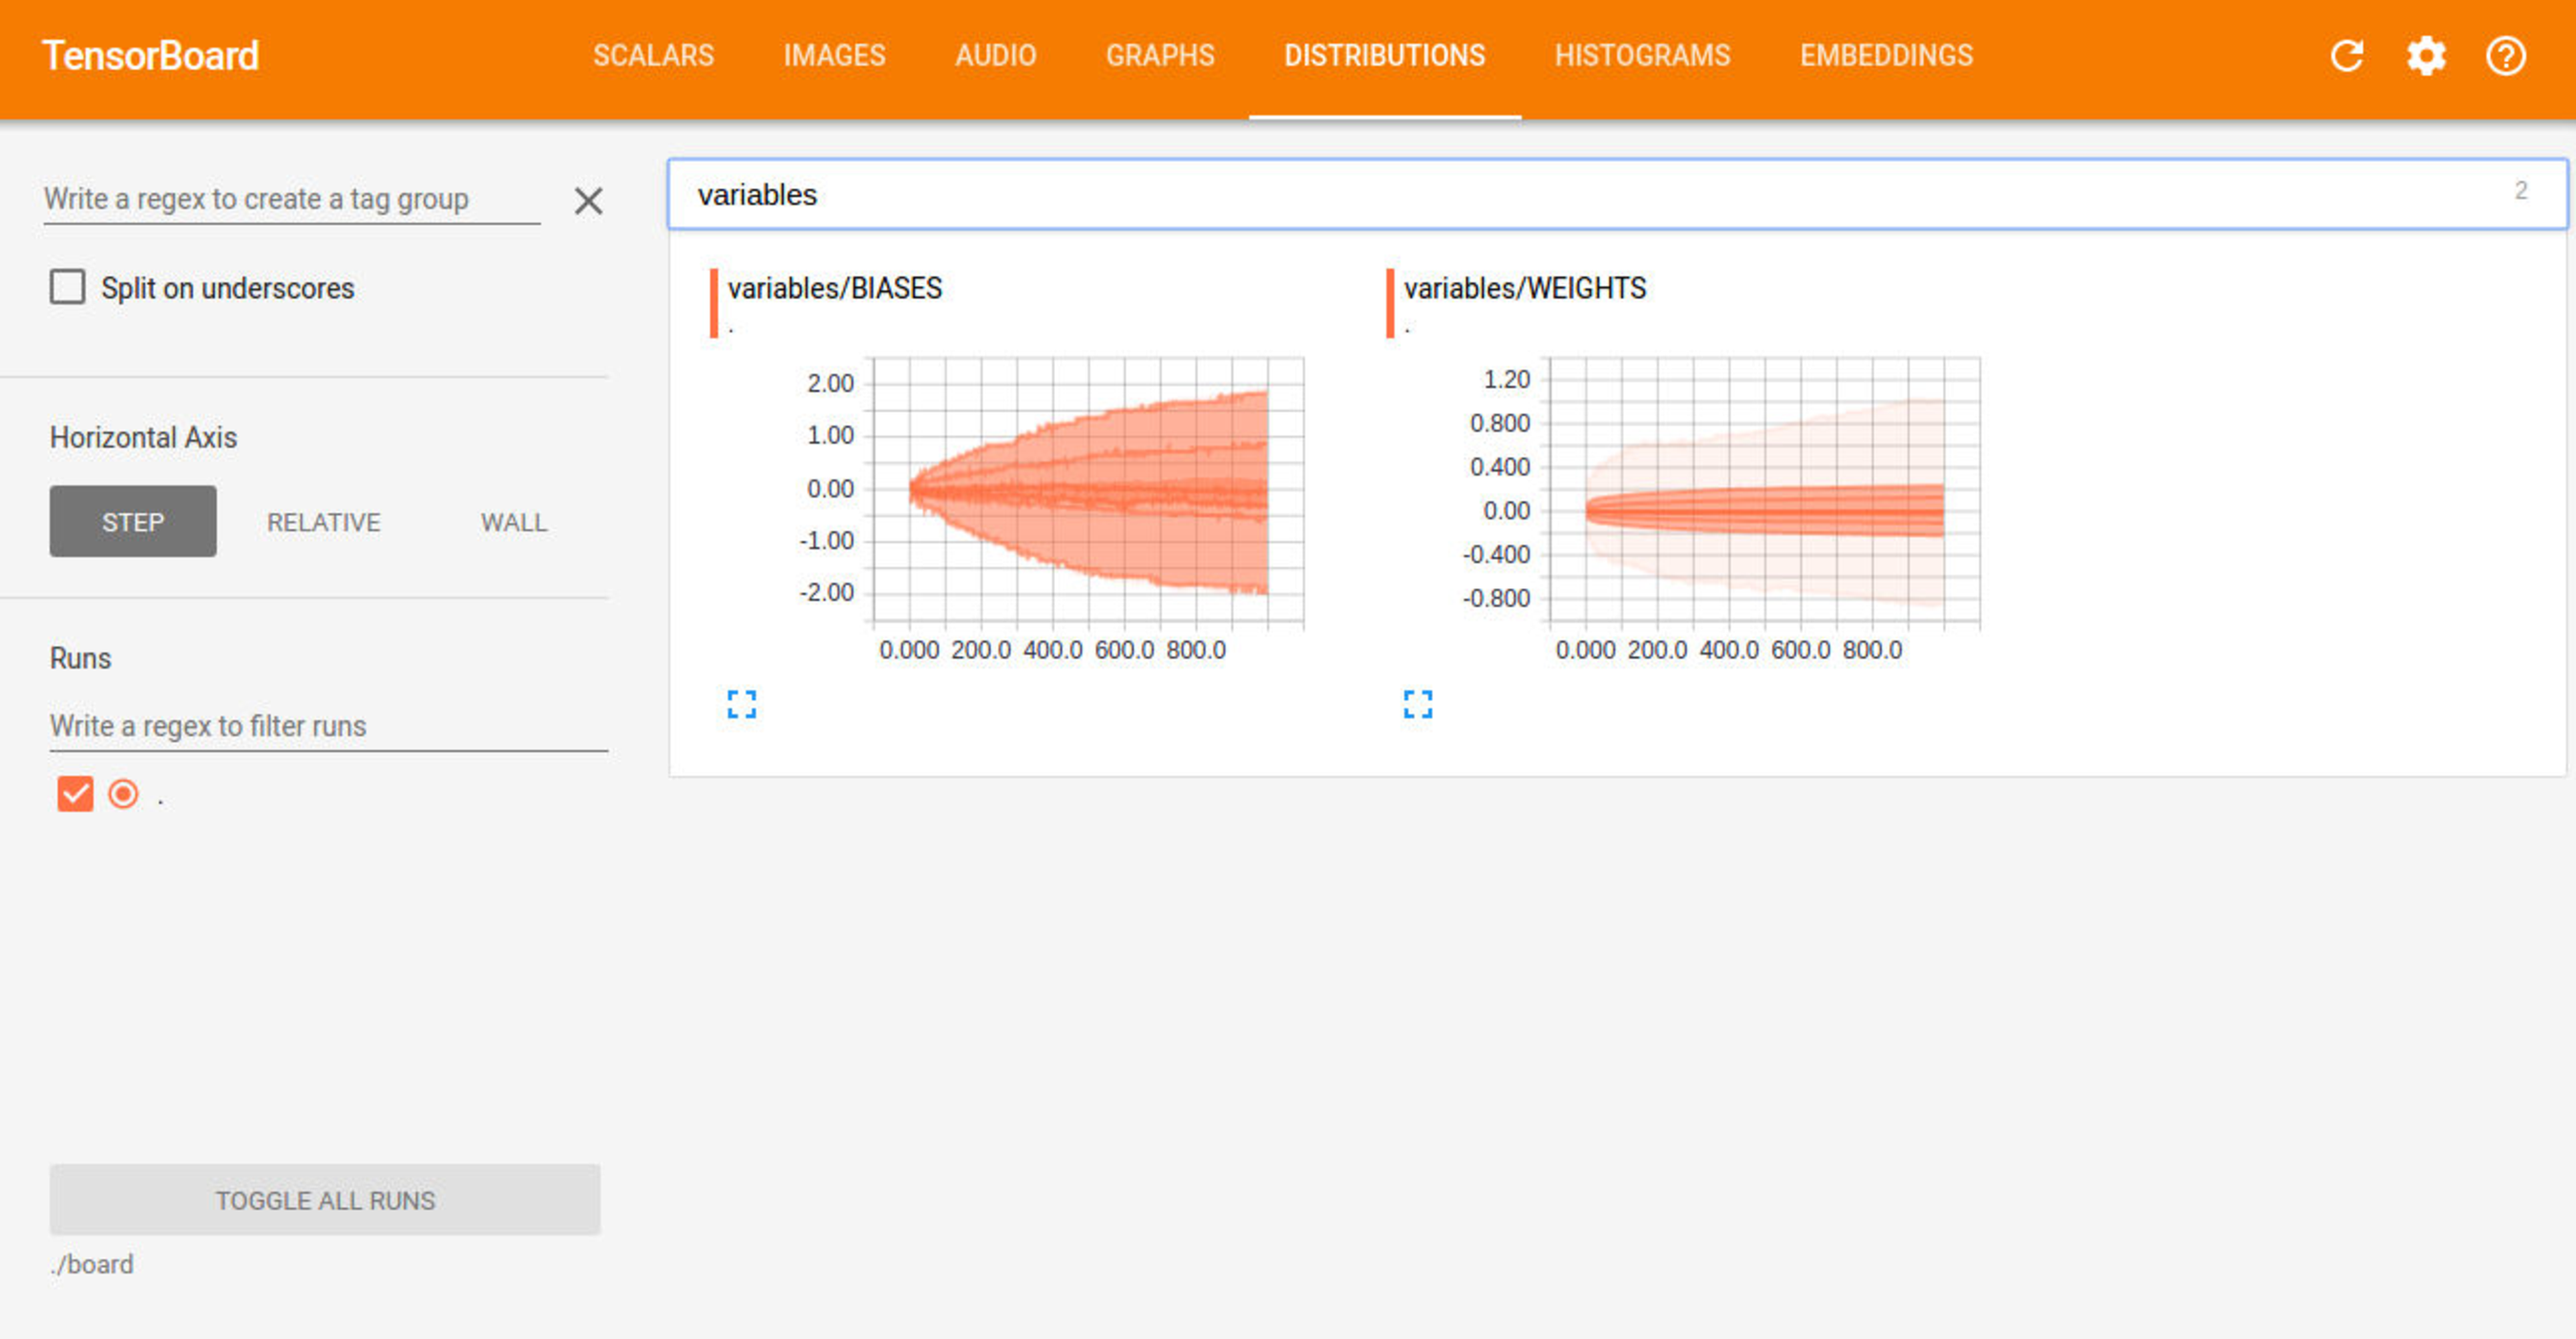
\includegraphics[width=0.95\paperwidth]{figures/distributions.pdf} 
	
\end{frame}

%

\begin{frame}
	\MyLogo
	\frametitle{TensorBoard: Histograms}  
	
\centering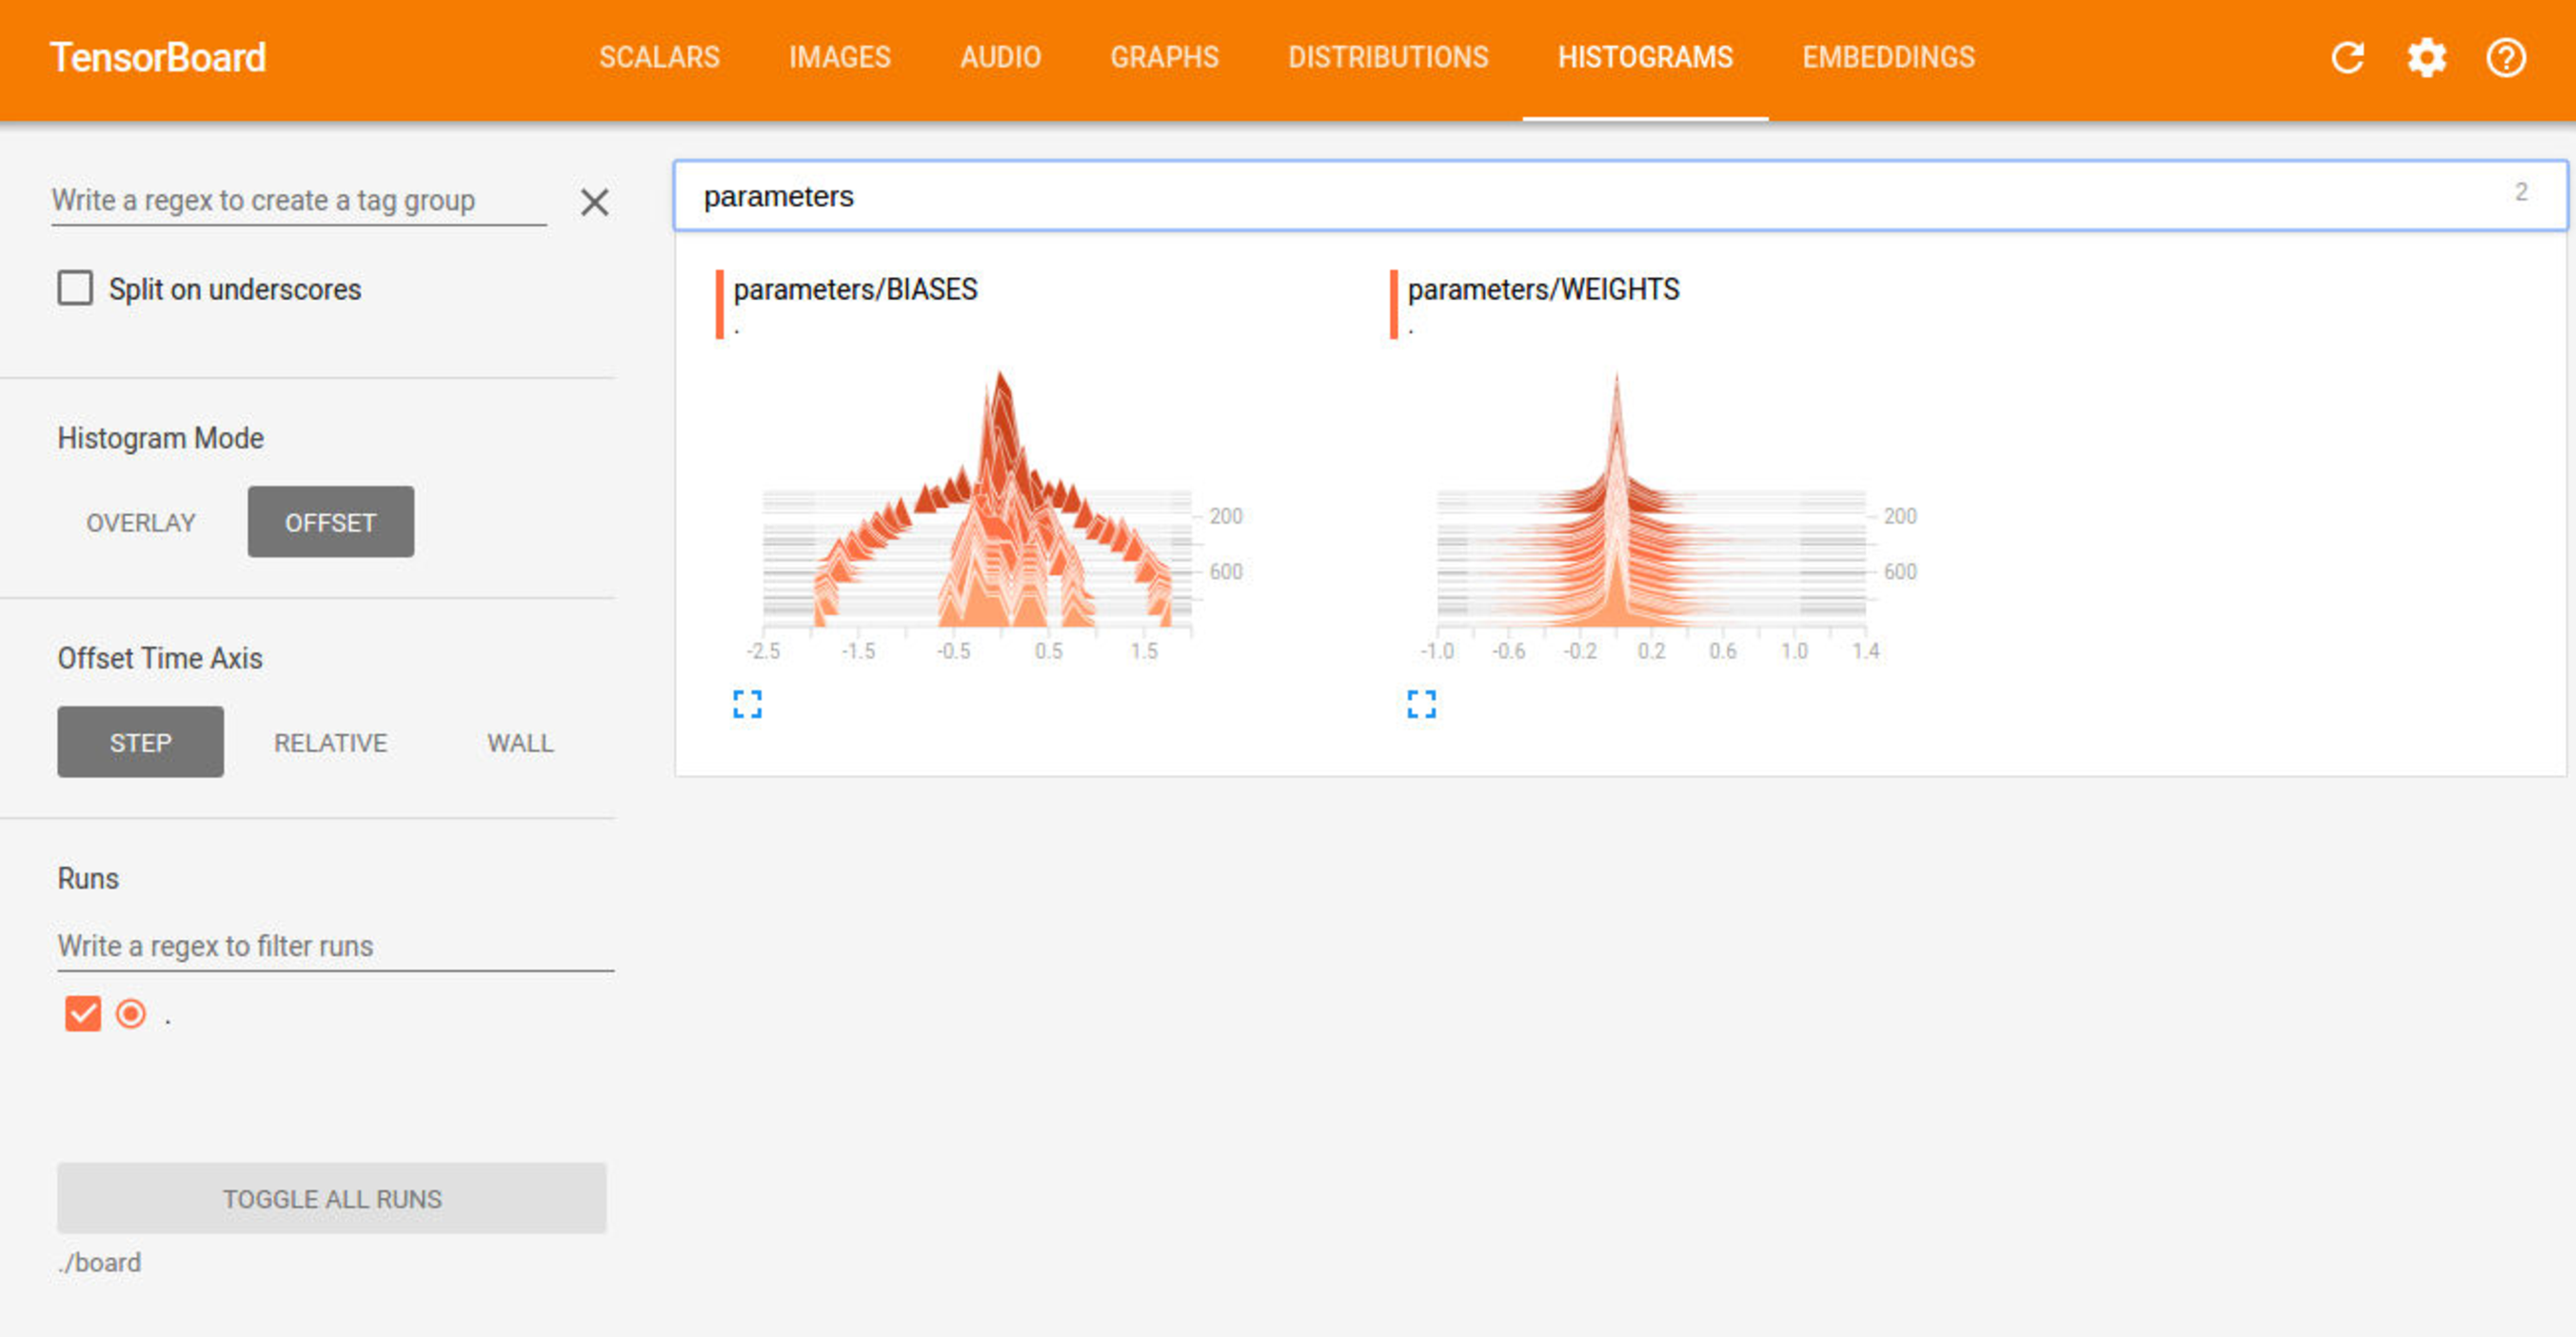
\includegraphics[width=0.95\paperwidth]{figures/histograms.pdf} 
	
\end{frame}